\documentclass{fenicscourse}

\begin{document}

\fenicslecture{Lecture 9: Incompressible Navier--Stokes}{Anders Logg \\ Marie E. Rognes}


%\begin{frame}
  \frametitle{The incompressible Navier--Stokes equations}

  \vspace{-0.5cm}

  \begin{alignat*}{2}
    \rho (\dot{u} + u \cdot \nabla u)
    - \nabla \cdot \sigma(u, p) &= f && \quad \text{ in } \Omega \times (0, T] \\
    \nabla \cdot u &= 0 && \quad \text{ in } \Omega \times (0, T] \\
    u &= g_{_\mathrm{D}} && \quad \text{ on } \Gamma_{_\mathrm{D}} \times (0, T] \\
    \sigma \cdot n &= t_{_\mathrm{N}} && \quad \text{ on } \Gamma_{_\mathrm{N}} \times (0, T] \\
    u(\cdot, 0) &= u_0 && \quad \text{ in } \Omega
  \end{alignat*}

  \linespread{1}
  \begin{itemize}
  \item
    $u : \Omega \rightarrow \R^d$ is the fluid velocity and $p : \Omega \rightarrow \R$ is the pressure
  \item
    $\rho$ is the fluid density
  \item
    $\sigma(u, p) = 2\mu\epsilon(u) - pI$ is the Cauchy stress tensor
  \item
    $\epsilon(u) = \frac{1}{2}(\nabla u + \nabla u^{\top})$ is the
    strain rate tensor
  \item
    $f$ is a given body force per unit volume
  \item
    $g_{_\mathrm{D}}$ is a given boundary velocity
  \item
    $t_{_\mathrm{N}}$ is a given boundary traction
  \item
    $u_0$ is a given initial velocity
  \end{itemize}
  \linespread{1.5}

\end{frame}
 % More compact (v1)
  \begin{frame}

  \frametitle{Definitions}

    \begin{itemize}
    \item
      Let $\Omega$ be a domain in $\R^d$ ($d = 1, 2, 3$) with coordinates $x$
    \item
      The boundary is $\partial \Omega = \Gamma_{_\mathrm D} \cup
      \Gamma_{_\mathrm N}$, $\Gamma_{_\mathrm D} \cap \Gamma_{_\mathrm
        N} = \emptyset$
    \item
      $u : \Omega \rightarrow \R^d$ is the \alert{unknown} fluid velocity
    \item
      $p : \Omega \rightarrow \R$ is the \alert{unknown} fluid pressure
    \item
      $\nabla u = \{ \frac{\partial u_j}{\partial x_i}\}_{i, j=1}^{d}$ \alert{NB!}
    \item
      $\varepsilon(u) = \frac{1}{2}(\nabla u + \nabla u^{\top})$ is
      the strain rate tensor
    \item
      $\sigma(u, p) = 2\mu\varepsilon(u) - pI$ is the Cauchy stress tensor
    \item
      $\rho \in \R$ is a given fluid density
    \item
      $f$ is a given body force per unit volume
    \item
      $g_{_\mathrm{D}}$ is a given boundary velocity
    \item
      $t_{_\mathrm{N}}$ is a given boundary traction
    \item
      $u_0$ is a given initial velocity
    \end{itemize}
\end{frame}
 % Less compact (v2)
\begin{frame}
  \frametitle{The incompressible Navier--Stokes equations}

  Constitutive equations
  \begin{alignat*}{2}
    \rho (\dot{u} + u \cdot \nabla u)
    - \nabla \cdot \sigma(u, p) &= f && \quad \text{ in } \Omega \times (0, T] \\
      \nabla \cdot u &= 0 && \quad \text{ in } \Omega \times (0, T]
  \end{alignat*}
  Boundary conditions
  \begin{alignat*}{2}
    u &= g_{_\mathrm{D}} && \quad \text{ on } \Gamma_{_\mathrm{D}} \times (0, T] \\
    \sigma \cdot n &= t_{_\mathrm{N}} && \quad \text{ on } \Gamma_{_\mathrm{N}} \times (0, T]
  \end{alignat*}
  Initial condition
  \begin{equation*}
    u(\cdot, 0) = u_0 \quad \text{ in } \Omega
  \end{equation*}


  \end{frame}
             % Less compact (v2)
\begin{frame}
  \frametitle{Mixed variational formulation of Navier--Stokes}

  Multiply the \alert{momentum equation} by a test function $v$ and
  integrate by parts:
  \begin{equation*}
    \int_{\Omega} \rho (\dot{u} + u \cdot \nabla u) \cdot v \dx
    + \int_{\Omega} \sigma(u, p) : \varepsilon(v) \dx
    = \int_{\Omega} f \cdot v \dx
    + \int_{\Gamma_{_\mathrm{N}}} t_{_{\mathrm{N}}} \cdot v \ds
  \end{equation*}
  Short-hand notation: $\inner{\cdot}{\cdot}$ is $L^2$-inner product
  \begin{equation*}
    \inner{\rho \dot{u}}{v} + \inner{\rho u \cdot \nabla u}{v}
    + \inner{\sigma(u, p)}{\varepsilon(v)}
    = \inner{f}{v}
    + \inner{t_{_{\mathrm{N}}}}{v}_{\Gamma_{_{\mathrm{N}}}}
  \end{equation*}

  \bigskip

  Multiply the \alert{continuity equation} by a test function $q$ and
  sum up: find $(u, p) \in V$ such that
  \begin{align*}
    \inner{\rho \dot{u}}{v} + \inner{\rho u \cdot \nabla u}{v}
    + \inner{\sigma(u, p)}{\varepsilon(v)}
    + \inner{\nabla \cdot u}{q}
    &= \inner{f}{v} + \inner{t_{_{\mathrm{N}}}}{v}_{\Gamma_{_{\mathrm{N}}}}
  \end{align*}
  for all $(v, q) \in \hat{V}$

\end{frame}

\begin{frame}
  \frametitle{Discrete mixed variational form of Navier--Stokes}

  Time-discretization leads to a \emph{saddle-point} problem on each time step:
  \begin{equation*}
    \left[
      \begin{array}{cc}
        M + \Delta t A + \Delta t N(U) & \Delta t B \\
        \Delta t B^{\top} & 0
      \end{array}
    \right]
    \left[
      \begin{array}{c}
        U \\ P
      \end{array}
    \right]
    =
    \left[
      \begin{array}{c}
        b\\ 0
      \end{array}
    \right]
  \end{equation*}

  \begin{itemize}
  \item
    Efficient solution of the saddle-point problem relies on the
    efficiency of special-purpose preconditioners (Uzawa iteration,
    Schur complement preconditioners, \ldots)
  \item
    We will use another approach (simpler and often more efficient)
  \end{itemize}

\end{frame}

\begin{frame}
  \frametitle{Splitting scheme for Navier-Stokes: Core idea}
  \begin{itemize}
  \item
    Solving the full coupled system for the velocity and the pressure
    simultaneously is computationally expensive.
  \item
    To reduce computational cost, iterative \emph{splitting schemes}
    are an attractive alternative.
  \item
    Splitting schemes are typically based on solving for the velocity
    and the pressure separately.
  \item
    We will consider a splitting scheme solving three different
    (smaller!) systems at each time step $n$:
    \begin{enumerate}
    \item
      Compute the \emph{tentative velocity}
    \item
      Compute the \emph{pressure}
    \item
      Compute the \emph{corrected velocity}
    \end{enumerate}
  \item
    Next slides show how the scheme is derived -- time to pay close attention!
  \end{itemize}
\end{frame}

\begin{frame}
  \frametitle{A splitting scheme for Navier--Stokes (Part 1/3)}

  \vspace{1em}
  Recall momentum equation:
  \begin{equation*}
    \rho (\dot{u} + u \cdot \nabla u) - \nabla \cdot \sigma(u, p) = f
  \end{equation*}

  Consider a time step $(t_{n-1}, t_{n})$ of length $k_n = t_{n} -
  t_{n-1}$, and introduce
  \begin{equation*}
  \dot{u}(t^n) \approx D_t u^n \equiv (u^n - u^{n-1}) / k_n
  \end{equation*}

  \medskip

  \alert{Assume $u^{n-1}$ is given, want to compute $u^{n}$}.

  \medskip

  A Crank-Nicolson approximation with explicit convection for the
  time-discretization gives
  \begin{equation*}
    \rho D_t u^n + \rho u^{n-1} \cdot \nabla u^{n-1}
    - \nabla \cdot \sigma(u^{n-1/2}, p^{n-1/2})
    = f^{n-1/2}
  \end{equation*}

  Define the \alert{tentative velocity} $u^{\bigstar}$ using
  the approximation
  \begin{equation}
    \rho D_t u^{\bigstar} + \rho u^{n-1} \cdot \nabla u^{n-1}
    - \nabla \cdot \sigma(u^{n-1/2}, \textcolor{red}{p^{n-3/2}})
    = f^{n-1/2}
  \end{equation}

\end{frame}

\begin{frame}
  \frametitle{A splitting scheme for Navier-Stokes (Part 2/3)}

  \vspace{1em}
  Subtract the equation for the tentative velocity from the equation
  for the \alert{corrected velocity} $u^n$:
  \begin{equation*}
    \rho (D_t u^n - D_t u^{\bigstar})
    - \nabla \cdot \sigma(0, p^{n-1/2} - p^{n-3/2})
    = 0
  \end{equation*}

  Definition of $D_t$ gives:
  \begin{equation*}
    \rho (D_t u^n - D_t u^{\bigstar})
    = \rho \left ( \frac{u^n - u^{n-1}}{k_n} - \frac{u^{\bigstar} - u^{n-1}}{k_n} \right )
    = \frac{\rho}{k_n}(u^n - u^{\bigstar})
    \end{equation*}

  Definition of $\sigma(u, p) = 2 \mu \varepsilon (u) - p I $ gives:
  \begin{equation*}
  \begin{split}
    - \nabla \cdot \sigma(0, p^{n-1/2} - p^{n-3/2})
    &=  \nabla \cdot (p^{n-1/2} - p^{n-3/2}) I \\
    &=  \nabla (p^{n-1/2} - p^{n-3/2})
  \end{split}
  \end{equation*}

  Multiplying by $k_n$ and keeping only $u^n$ on the left hand side give
  \begin{equation}
    \rho u^n = \rho u^{\bigstar} - k_n \nabla (p^{n-1/2} - p^{n-3/2})
    \label{eq:velocitycorrection}
  \end{equation}

  \end{frame}



\begin{frame}
  \frametitle{A splitting scheme for Navier-Stokes (Part 3/3)}

  \vspace{1em}
  Recall~\eqref{eq:velocitycorrection}:
  \begin{equation*}
    \rho u^n = \rho u^{\bigstar} - k_n \nabla (p^{n-1/2} - p^{n-3/2})
  \end{equation*}

  Assuming $u^{\bigstar}$ and $p^{n - 3/2}$ given, \alert{need $p^{n-1/2}$!}

  \bigskip

  Taking the divergence of~\eqref{eq:velocitycorrection} gives
  \begin{equation*}
    \rho \nabla \cdot u^n  = \nabla \cdot \left ( \rho u^{\bigstar} - k_n \nabla (p^{n-1/2} - p^{n-3/2}) \right )
  \end{equation*}

  We want $\nabla \cdot u^n = 0$, i.e
  \begin{equation*}
    0  = \nabla \cdot \left ( \rho u^{\bigstar} - k_n \nabla (p^{n-1/2} - p^{n-3/2}) \right )
  \end{equation*}
  or equivalently (denoting $\Delta p = \nabla \cdot \nabla p$):
  \begin{equation}
    - k_n \Delta p^{n-1/2} = -k_n \Delta p^{n-3/2} - \rho \nabla \cdot u^{\bigstar}
    \label{eq:pressurecorrection}
  \end{equation}
\end{frame}


\begin{frame}
\frametitle{A splitting scheme for Navier-Stokes (Summary)}

For each $n$, given $u^{n-1}$ and $p^{n-3/2}$,
\medskip
\begin{itemize}
\item
  \textbf{Step 1}: Compute the tentative velocity $u^{\bigstar}$ from
  \begin{equation*}
    \rho D_t u^{\bigstar} + \rho u^{n-1} \cdot \nabla u^{n-1}
    - \nabla \cdot \sigma(u^{n-1/2}, p^{n-3/2})
    = f^{n-1/2}
  \end{equation*}
  \item
    \textbf{Step 2}: Compute the pressure $p^{n - 1/2}$ from
    \begin{equation*}
      - k_n \Delta p^{n-1/2} = -k_n \Delta p^{n-3/2} - \rho \nabla \cdot u^{\bigstar}
    \end{equation*}
  \item
  \textbf{Step 3}: Compute the corrected velocity $u^{n}$ from
  \begin{equation*}
    \rho u^n = \rho u^{\bigstar} - k_n \nabla (p^{n-1/2} - p^{n-3/2})
  \end{equation*}
\end{itemize}
\end{frame}

%\begin{frame}
  \frametitle{Boundary conditions}

  \begin{itemize}
  \item
    No-slip boundary conditions ($u = g_D$ on $\Gamma_D$) are enforced
    strongly, i.e as Dirichlet boundary conditions.
  \item
    For outflow boundary conditions, corresponding to so-called
    ``do-nothing'' boundary conditions for the Laplacian formulation,
    we take $\partial_n u = 0$:
    \begin{align*}
      \sigma(u, p) \cdot n
      &= (2\mu \epsilon(u) - pI) \cdot n
      = \mu\nabla u \cdot n + \mu(\nabla u)^{\top} \cdot n - pn \\
      &= \mu\nabla u \cdot n - pn
      \approx \mu\nabla u^{n-1/2} \cdot n - p^{n-3/2}n
    \end{align*}
  \end{itemize}

  \begin{itemize}
  \item
    Boundary conditions for the pressure Poisson problem:
    \begin{equation*}
      \partial_n \dot{p} = 0
    \end{equation*}
    on the pressure Neumann boundary
  \end{itemize}

\end{frame}
 % More mysterious (v1)
\begin{frame}
  \frametitle{Boundary conditions}

  \vspace{1em}
  We consider boundary conditions of the type
  \begin{alignat*}{2}
    u &= g_{_\mathrm{D}} && \quad \text{ on } \Gamma_{_\mathrm{D}} \times (0, T] \\
    \sigma \cdot n &= t_{_\mathrm{N}} = - \bar{p} n  && \quad \text{ on } \Gamma_{_\mathrm{N}} \times (0, T]
  \end{alignat*}

  \begin{itemize}
  \item
    Velocity boundary conditions ($u = g_D$ on $\Gamma_D$) are
    enforced strongly in the finite element spaces, i.e as Dirichlet
    boundary conditions.
  \item
    Traction boundary conditions ($\sigma \cdot n = t_{_\mathrm{N}}$)
    are enforced weakly in the variational formulation.
  \end{itemize}

  In the splitting scheme, auxilliary boundary conditions are
  required for the pressure Poisson problem:
  \begin{align*}
    p &= \bar{p} \quad \text{ on } \Gamma_{_\mathrm{N}} \\
    \partial_n \dot{p} &= 0 \quad \text{ on } \Gamma_{_\mathrm{D}}
  \end{align*}
  and an auxiliary initial condition for the pressure $p^{-1/2} = p_0$.

\end{frame}

\begin{frame}
  \frametitle{Enforcing traction boundary conditions in splitting scheme}
  Note that
  \begin{equation*}
    \begin{split}
      \sigma(u^{n-1/2}, p^{n-3/2})
      &= 2 \mu \varepsilon (u^{n-1/2})  - p^{n-3/2} I - p^{n-1/2} I + p^{n-1/2} I \\
      &= \sigma(u^{n-1/2}, p^{n-1/2}) + p^{n-1/2} - p^{n-3/2}
    \end{split}
  \end{equation*}
  If we want to enforce
  \begin{equation*}
    \sigma(u^{n-1/2}, p^{n-1/2}) \cdot n = - \bar{p} n
  \end{equation*}
  and
  \begin{equation*}
    p^{n - 1/2} \cdot n = \bar{p} n
  \end{equation*}

  Then, we should say
  \begin{equation*}
    \sigma(u^{n-1/2}, p^{n-3/2}) \cdot n = - p^{n-3/2} n
  \end{equation*}
\end{frame}
 % Less mysterious (v2)

%\begin{frame}
  \frametitle{Incremental pressure correction scheme (IPCS)}

  For each $n$, given $u^{n-1}$ and \alert{$p^{n-3/2}$}:
  \begin{enumerate}
  \item
    Compute the tentative velocity $u^\bigstar$ by
    \begin{multline*}
      \inner{\rho D_t^n u^{\bigstar}}{v}
      + \inner{\rho u^{n-1} \cdot \nabla u^{n-1}}{v}
      + \inner{\sigma(u^{n-\frac{1}{2}}, p^{n-3/2})}{\epsilon(v)} \\
      - \inner{\mu \nabla u^{n-\frac{1}{2}} \cdot n}{v}_{\partial\Omega}
      + \inner{p^{n-3/2} n}{v}_{\partial\Omega}
      = \inner{f^{n-1/2}}{v}
    \end{multline*}
  \item
    Compute the corrected pressure $p^{n-1/2}$ by
    \begin{equation*}
      k_n \inner{\nabla p^{n-1/2}}{\nabla q}
      = k_n \inner{\nabla p^{n-3/2}}{\nabla q}
      - \inner{\rho \nabla \cdot u^{\bigstar}}{q}
    \end{equation*}
  \item
    Compute the corrected velocity $u^n$ by
    \begin{equation*}
      \inner{\rho u^n}{v} = \inner{\rho u^{\bigstar}}{v}
      - k_n\inner{\nabla(p^{n-1/2} - p^{n-3/2})}{v}
    \end{equation*}
  \end{enumerate}

\end{frame}
 % v1
\begin{frame}
  \frametitle{Weak formulation of N-S splitting scheme}

  \vspace{0.5em}
  For $n = 1, 2, \dots, N$, given $u^{0}$ and $p^{-1/2}$:
  \begin{enumerate}
  \item
    Compute $u^\bigstar$ with $u^{\bigstar}|_{\Gamma_{_\mathrm D}} =
    g_{_\mathrm D}$ solving
    \begin{equation*}
      \begin{split}
        \inner{\rho D_t^n u^{\bigstar}}{v}
        + \inner{\rho u^{n-1} \cdot \nabla u^{n-1}}{v}
        + \inner{\sigma(u^{n-\frac{1}{2}}, p^{n-3/2})}{\varepsilon(v)} \\
        = \inner{f^{n-1/2}}{v}
        - \inner{p^{n-3/2} n}{v}_{\partial \Omega}
      \end{split}
    \end{equation*}
    for all $v$ such that $v|_{\Gamma_{_\mathrm D}} = 0$.
  \item
    Compute $p^{n-1/2}$ with $p^{n-1/2}|_{\Gamma_{_\mathrm N}} = \bar{p}$
    \begin{equation*}
      k_n \inner{\nabla p^{n-1/2}}{\nabla q}
      = k_n \inner{\nabla p^{n-3/2}}{\nabla q}
      - \inner{\rho \nabla \cdot u^{\bigstar}}{q}
    \end{equation*}
    for all $q$ such that $q|_{\Gamma_{_\mathrm N}} = 0$
  \item
    Compute $u^{n}$ solving
    \begin{equation*}
      \inner{\rho u^n}{v} = \inner{\rho u^{\bigstar}}{v}
      - k_n\inner{\nabla(p^{n-1/2} - p^{n-3/2})}{v}
    \end{equation*}
    for all $v$.
  \end{enumerate}

\end{frame}
 % v2
\begin{frame}[fragile]
  \frametitle{Useful FEniCS tools (I)}

  Note $\Grad$ vs. $\nabla$:
  \vspace{-1em}
  \begin{python}
dot(grad(u), u)
dot(u, nabla_grad(u))
  \end{python}

  \bigskip

  Defining operators:
  \vspace{-1em}
  \begin{python}
def sigma(u, p):
    return 2.0*mu*sym(grad(u))-p*Identity(len(u))
  \end{python}

  \bigskip

  The facet normal $n$:
  \vspace{-1em}
  \begin{python}
n = FacetNormal(mesh)
  \end{python}

\end{frame}

\begin{frame}[fragile]
  \frametitle{Useful FEniCS tools (II)}

  \linespread{1.0}

  Assembling matrices and vectors:
  \vspace{-0.5cm}
  \begin{python}
A = assemble(a)
b = assemble(L)
  \end{python}

  \smallskip

  Solving linear systems:
  \vspace{-0.5cm}
  \begin{python}
solve(A, x, b)
solve(A, x, b, "gmres", "ilu")
solve(A, x, b, "cg", "amg")
  \end{python}

  \smallskip

  Extracting left- and right-hand sides:
  \vspace{-0.5cm}
  \begin{python}
F = <complicated expression>
a = lhs(F)
L = rhs(F)
  \end{python}

\end{frame}

\begin{frame}
  \frametitle{\emph{The FEniCS challenge!}}

  \linespread{1.5}

  Solve the incompressible Navier--Stokes equations for the flow of
  water around a dolphin. The water is initially at rest and the flow
  is driven by a pressure gradient.

  \begin{center}
    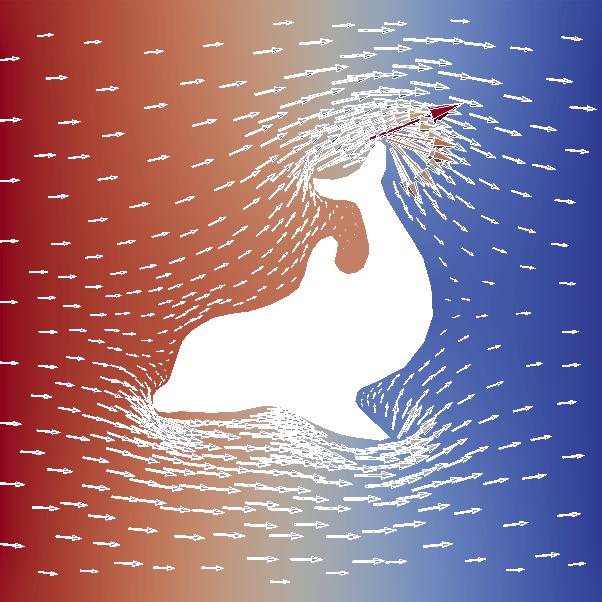
\includegraphics[width=0.5\textwidth]{png/dolfin_channel.png}
  \end{center}

\end{frame}

\begin{frame}[fragile]
  \frametitle{\emph{The FEniCS challenge!}}

  \begin{itemize}
  \item
    Use the mesh \texttt{dolfin\_channel.xml.gz}, and finite element
    spaces $V_h = \mathcal{P}_2^2$ and $Q_h = \mathcal{P}_1$
  \item
    Compute the solution on the time interval $[0, 0.1]$ with time
    steps of size $k = 0.0005$
  \item
    Set $\bar{p} = 1~\mathrm{kPa}$ at the inflow (left side) and
    $\bar{p} = 0$ at the outflow (right side)
  \item
    Set $g_{_\mathrm{D}} = (0, 0)$ on the remaining boundary
  \item
    Set $f = (0, 0)$
  \item
    The density of water is $\rho = 1000~\mathrm{kg} / \mathrm{m}^3$ and
    the viscosity is $\mu = 0.001002~\mathrm{kg} / (\mathrm{m \cdot s})$
  \item
    To check your answer, compute the average velocity in the $x$-direction:
    \begin{equation*}
      \bar u_x = \tfrac{1}{|\Omega|} \int_{\Omega} u \cdot (1, 0) \dx
    \end{equation*}
  \end{itemize}

  \bigskip

  \emph{The student(s) who first produce the right answer will be
    rewarded with an exclusive FEniCS surprise!}

\end{frame}



\end{document}
